\documentclass{article}
\usepackage[utf8]{inputenc}
\usepackage[catalan]{babel}
\usepackage{amssymb}        % símbols de l'AMS
\usepackage{amsmath}        % macros de l'AMS
\usepackage[pdftex]{graphicx}  % poder incloure gráfics
\usepackage[pdftex]{color}     % poder fer servir color al text
\usepackage{multicol}
\usepackage{amsthm}
\usepackage{listings}
\usepackage{hyperref}
\usepackage{geometry}
\usepackage{tikz}
\usepackage{pgfplots}
\usepackage{subcaption}
\usepackage[catalan]{babel}
\usepackage{mathtools}
\usepackage{geometry}
\usepackage{amsmath}
\usepackage{amssymb}
\usepackage{fancyhdr}
\usepackage{multirow}
%\usepackage[table,xcdraw]{xcolor}
\usepackage{float}
\usepackage{verbatim}
\usepackage{pgfplots}
\pgfplotsset{compat=newest}
\usepgfplotslibrary{fillbetween}
\usetikzlibrary{patterns}
\usepackage{vmargin} 				%margenes



\title{Pràctica 2: Classificació}
\author{Guillermo Vivancos Alonso 1606206\\
	Javier Esmoris Cerezuela 1498396\\
	Oriol Marión Escudé 1566740}
\begin{document}
	\date{}
	\setpapersize{A4}
	\setmargins{2.5cm}       % margen izquierdo
	{1.5cm}                        % margen superior
	{16.5cm}                      % anchura del texto
	{23.42cm}                    % altura del texto
	{10pt}                           % altura de los encabezados
	{1cm}                           % espacio entre el texto y los encabezados
	{0pt}                             % altura del pie de página
	{2cm}                           % espacio entre el texto y el pie de página
	
	\pagestyle{fancy}
	\fancyhf{}
	\lhead{\textbf{Aprenentatge Computacional 102787} \newline Pràctica 2: Classificació\\}
	\rhead{\hfill \textbf{
			Guillermo Vivancos Alonso 1606206\\
			Javier Esmoris Cerezuela 1498396\\
			Oriol Marión Escudé 1566740}}
	\rfoot{\thepage}
	\maketitle
	\noindent
	\section*{Introducció}
	En aquesta pràctica analitzarem una base de dades sobre la potabilitat de l'aigua i les diferents concentracions d'algunes substàncies. Veurem quines distribucions tenen els atributs, la relació entre ells i intentarem determinar si donada una mostra, aquesta és potable o no.
	
	\section*{Apartat B}
	\textbf{Exploratory Data Analysis}\\
	\\
	Els atributs que tenim a la base de dades són els següents:
	\begin{enumerate}
		\addtocounter{enumi}{-1}
		\item pH [float]: pH de l'aigua.
		\item Hardness [float]:concentració de calci i magnesi.
		\item Solids [float]: edat del jugador mesurada en anys i dies.
		\item Chloramines [float]: concentració de cloramines. 
		\item Sulfate [float]: concentració de sulfats.
		\item Conductivity [float]: conductivitat de l'aigua.
		\item Organic\_carbon [float]: concentració de compostos orgànics.
		\item Trihalomethanes [float]: concentració de trihalometans.
		\item Turbidity [float]: Terbolesa de l'aigua.
		\item Potability [integer]: 0 si no és potable, 1 si és potable.
	\end{enumerate}
	Tenim 10 atributs a la base de dades, tots de tipus float menys l'últim que és binari, per tant l'atribut categòric només pot prendre dos valors.\\
	\\
	Pel que fa a les correlacions amb l'atribut categòric, totes són poc significatives com es pot veure en la figura~\ref{fig:correlacions}.\\
	\begin{figure}[!h]
		\centering
		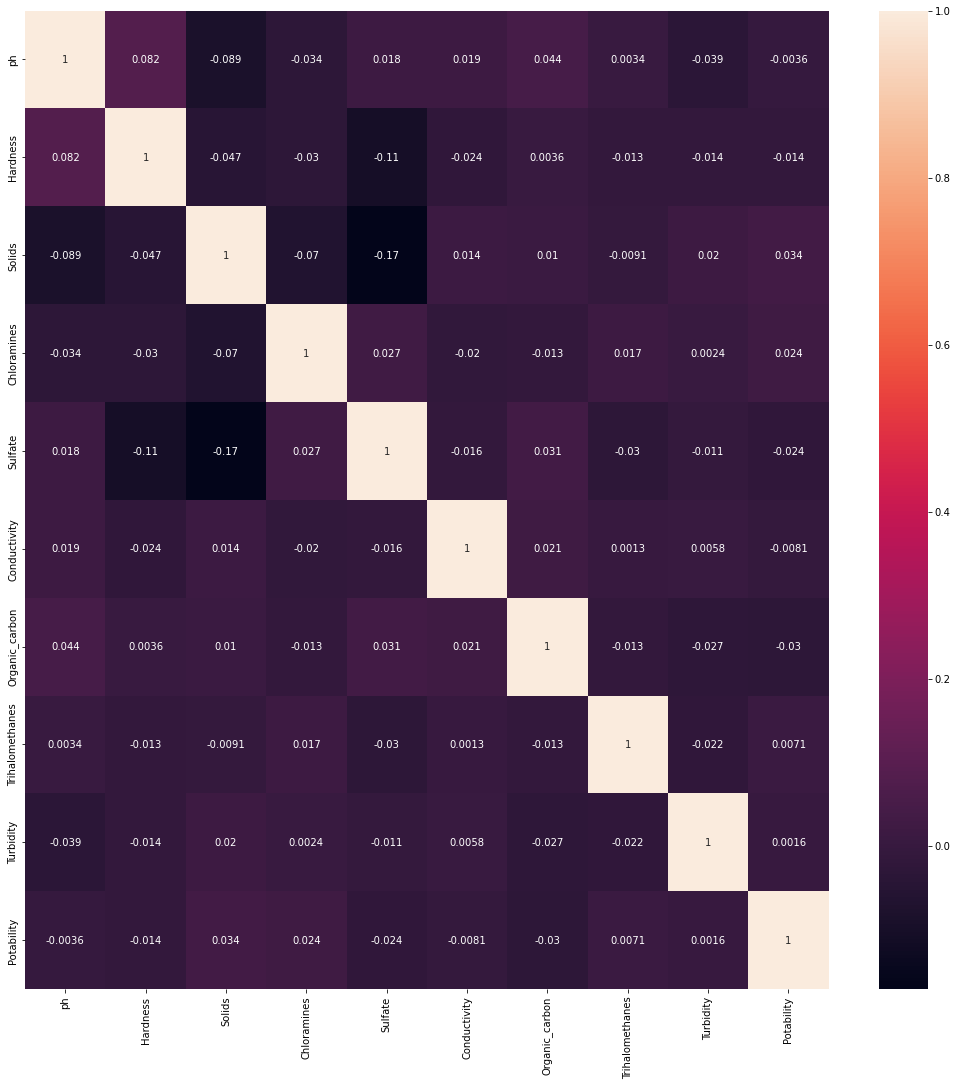
\includegraphics[width=0.4\linewidth]{../images/correlacions}
		\caption{Correlació entre els atributs}
		\label{fig:correlacions}
	\end{figure}\\
	A continuació veurem la distribució de la potabilitat~\ref{fig:distribuciopotabilitat} i les distribucions dels altres atributs segons la potabilitat~\ref{fig:distribucions}.\\
	\begin{figure}[!h]
		\centering
		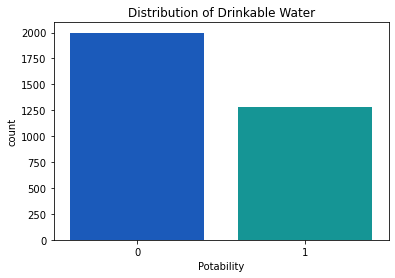
\includegraphics[width=0.4\linewidth]{../images/distribucio_potabilitat}
		\caption{Distribucio de la potabilitat}
		\label{fig:distribuciopotabilitat}
	\end{figure}
	\begin{figure}[!h]
		\centering
		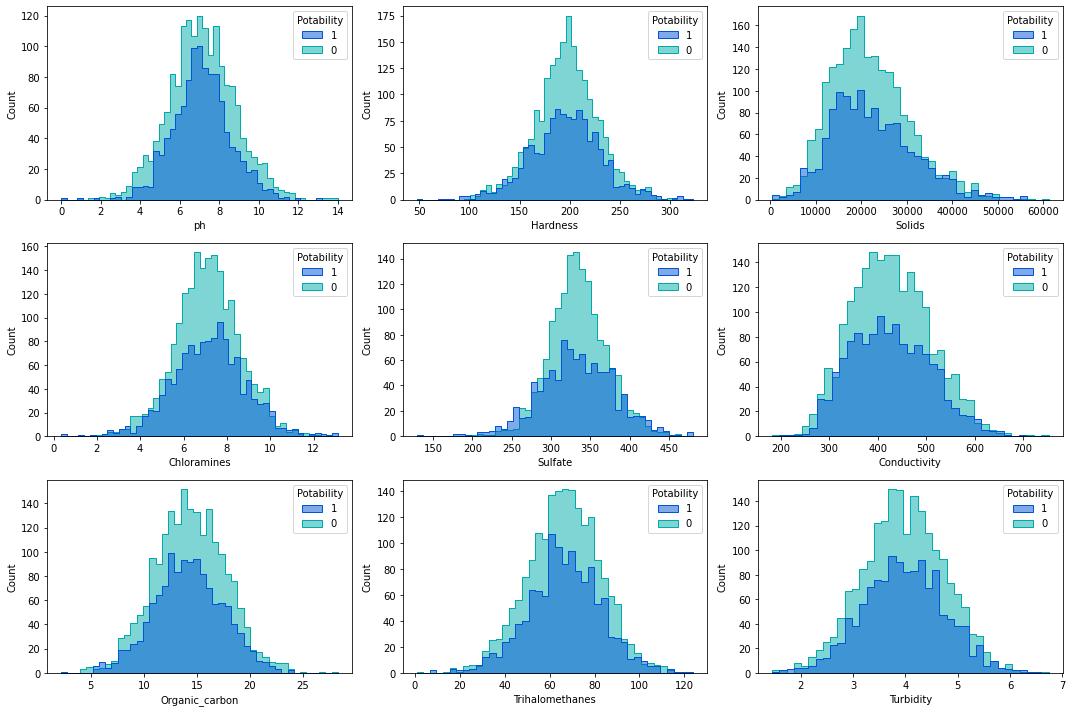
\includegraphics[width=0.7\linewidth]{../images/distribucions}
		\caption{Distribucions dels atributs segons la potabilitat}
		\label{fig:distribucions}
	\end{figure}\\
	A simple vista podem veure en la figura~\ref{fig:distribucions} que els atributs tenen una distribució gaussiana o pràcticament gaussiana. Les etiquetes de potabilitat estan balancejades (proporció 3:2).
	\clearpage
	\noindent
	\textbf{Preprocessing}\\
	\\
	En primer lloc mirem quines variables tenen NaNs, que són pH, Sulfate i Trihalomethanes. Els valors mitjans dels atributs, tant quan l'aigua és potable com no, són molt semblants, per tant, substituim els NaNs per la mitja dels atributs.\\
	\\
	La variable categòrica pren només dos valors, per tant tècniques com Ordinal Encoder o OneHotEncoder no tenen gaire sentit en aquest context.\\
	\\
	Hi ha rangs de variables molt aixos en comparació amb uns altres. L'atribut solids té el rang més alt de l'ordre de $6\cdot10^6$, mentre que el rang del pH és de 14 i el de Turbidity és de 3. És per això que cal normalitzar les dades. La normalització que hem fet servir és la estàndar.\\
	\\
	No tenim files repetides a la base de dades.\\
	\\
	\\
	\textbf{Model Selection}\\
	\\	
	Els models que hem fet són el knn amb $k=1..4$, regressió logística, SVM (lineal, polinomial, sigmoid, rbf), perceptró, random forest, bagging en decision trees i svc i, finalment, boosting.\\
	\begin{figure}[!h]
		\centering
		\begin{subfigure}[b]{0.25\textwidth}
			\centering
			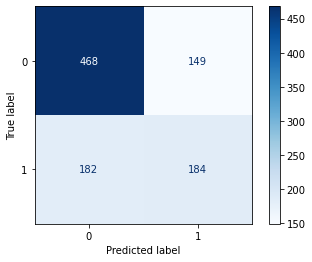
\includegraphics[width=\textwidth]{../images/cmatrix-knn}
			\caption*{Knn per $k=1..4$}
			\label{fig:knn}
		\end{subfigure}
		\hfill
		\begin{subfigure}[b]{0.25\textwidth}
			\centering
			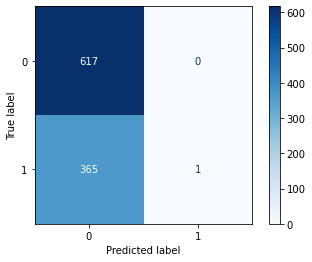
\includegraphics[width=\textwidth]{../images/cmatrix-logistic}
			\caption*{Regressió logística}
			\label{fig:three sin x}
		\end{subfigure}
		\hfill
		\begin{subfigure}[b]{0.25\textwidth}
			\centering
			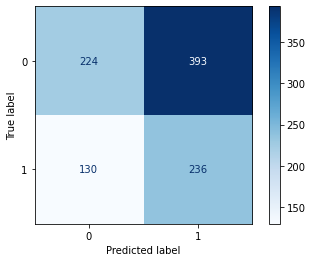
\includegraphics[width=\textwidth]{../images/cmatrix-perceptro}
			\caption*{Perceptró}
			\label{fig:five over x}
		\end{subfigure}
		\label{fig:three graphs}
	\end{figure}

\begin{figure}[!h]
	\centering
	\begin{subfigure}[b]{0.25\textwidth}
		\centering
		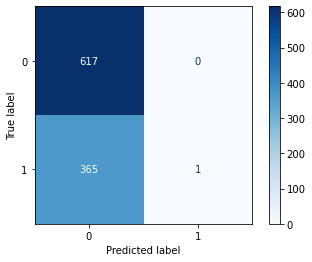
\includegraphics[width=\textwidth]{../images/cmatrix-svm-linear}
		\caption*{SVM linear kernel}
		\label{fig:knn}
	\end{subfigure}
	\hfill
	\begin{subfigure}[b]{0.25\textwidth}
		\centering
		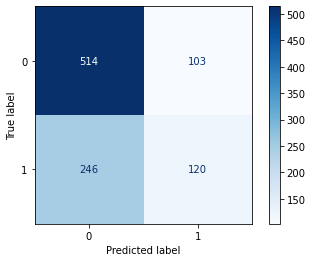
\includegraphics[width=\textwidth]{../images/cmatrix-svm-poly}
		\caption*{SVM polynomial kernel}
		\label{fig:three sin x}
	\end{subfigure}
	\hfill
	\begin{subfigure}[b]{0.25\textwidth}
		\centering
		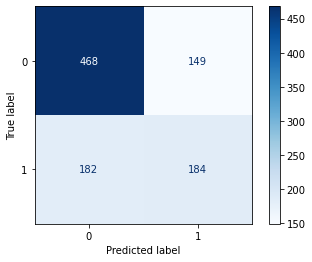
\includegraphics[width=\textwidth]{../images/cmatrix-svm-sigmoid-rbf}
		\caption*{SVM sigmoid or rbf kernel}
		\label{fig:five over x}
	\end{subfigure}
	\label{fig:three graphs}
\end{figure}
\begin{figure}[!h]
	\centering
	\begin{subfigure}[b]{0.25\textwidth}
		\centering
		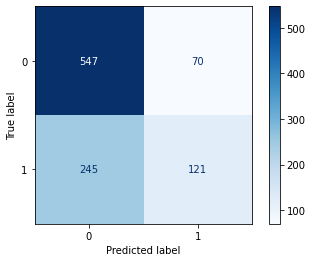
\includegraphics[width=\textwidth]{../images/cmatrix-random-forest}
		\caption*{Random forest}
		\label{fig:knn}
	\end{subfigure}
	\begin{subfigure}[b]{0.25\textwidth}
		\centering
		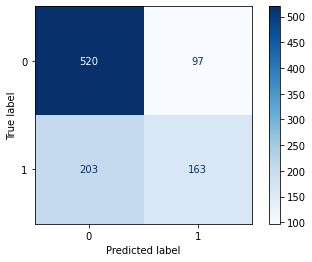
\includegraphics[width=\textwidth]{../images/cmatrix-bagging-decisiontrees}
		\caption*{Bagging en decision trees}
		\label{fig:three sin x}
	\end{subfigure}
\end{figure}
\begin{figure}[!h]
	\centering
	\begin{subfigure}[b]{0.25\textwidth}
		\centering
		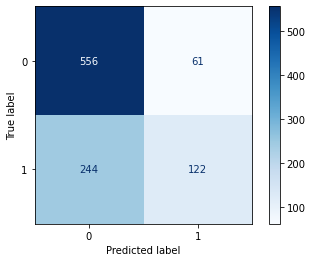
\includegraphics[width=\textwidth]{../images/cmatrix-bagging-svc}
		\caption*{Bagging en SVC}
		\label{fig:knn}
	\end{subfigure}
	\begin{subfigure}[b]{0.25\textwidth}
		\centering
		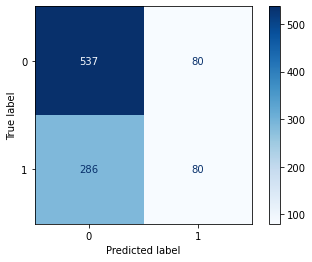
\includegraphics[width=\textwidth]{../images/cmatrix-boosting}
		\caption*{Boosting}
		\label{fig:three sin x}
	\end{subfigure}
\end{figure}
F1 scores obtinguts:\\
\begin{center}
	\begin{tabular}{|c|c|c|c|}\hline
		&SENSE PCA&		PCA&		PCA+POLYNOMIAL\\ \hline
		LOGISTIC REGRESSION& 0  & 0.005	& 0.46\\ \hline
		SVM	LINEAR& 0.005	& 0		& 0.31\\ \hline
		SVM POLY& 0.4	& 0.326	& 0.22\\ \hline
		SVM RBF& 0.52	&0.41	& 0.41\\ \hline
		SVM SIGMOID& 0.52	& 0.31	& 0.38\\ \hline
		KNN& 0.35		& 0.31	& 0.38\\ \hline
		PERCEPTRO& 0.47		& 0.47	& 0.47\\ \hline
		RF& 0.458		& 0.44	& 0.44\\ \hline
		BAGGING TREE &0.52	&0.52	& 0.48\\ \hline
		BAGGING: SVC & 0	& 0.44	&0.43\\ \hline
		BOOSTING& 0.3 & 0.3 & 0.47\\ \hline
	\end{tabular}
\end{center}
	\textbf{Crossvalidation}\\
	\\
	És molt important separar el conjunt d'entrenament del conjunt de test, ja que un model que sencillament repeteix les mateixes dades tindria un resultat perfecte, però no podrà predir res útil. Això es l'overfitting, per evitar-ho cross-validem els resultats per crear conjunts d'entrenament i conjunts de test diferents sobre un mateix model.\\
	\begin{figure}[!h]
		\centering
		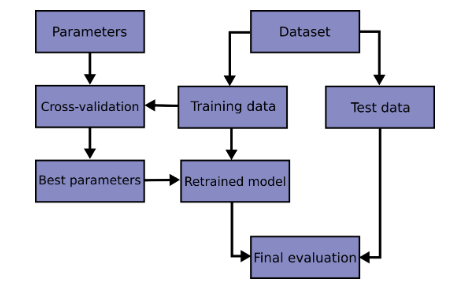
\includegraphics[width=0.4\linewidth]{../images/crossvalidation}
		\caption*{}
		\label{fig:crossvalidation}
	\end{figure}\\
	Els resultats seran millors amb un conjunt d'entrenament més gran fins a cert punt, amb poques dades d'entrenament l'accuracy serà menor i el volem el més alt possible, però si ens passem amb el tamany del conjunt d'entrenament podem arribar a comprometre els resultats, si les categories estan desbalancejades, o el rendiment.\\
	\\
	Hem fet servir el k-fold normal, en comparació amb el punt anterior hem aconseguit augmentar l'accuracy utilitzat k=5, aquest augmenta ja que hem entrenat el model amb 5 conjunts d'entrenament i test diferents\\
	\\
	No és eficient aplicar Leave-One-Out ja que prioritza que els conjunts d'entrenament siguin els més grans possibles, i en models amb moltes dades (+3000 en el nostre cas) compromet el rendiment consumint més temps del necessari.\\
	\\
	Hem calculat els accuracys per SVM, knn, regressió logística i random forest que són respectivament 0.61, 0.56, 0.61, 0.63.\\ 
	\\
	\textbf{Metric Analtyics}\\
	\\
	Vegem les mètriques pel SVM de rbf kernel, que és el que millor F1 score ens ha donat.\\
	\begin{center}
		\begin{tabular}{|c|c|c|c|c|}\hline
			&precision  &  recall & f1-score  & support\\ \hline
			
			Non-potable water   &    0.72 &     0.76 &     0.74 &      617\\ \hline
			Potable water    &   0.55    &  0.50     & 0.53      & 366\\ \hline
			
			accuracy       &     &          &     0.66     &  983\\ \hline
			macro avg       &0.64  &    0.63   &   0.63      & 983\\ \hline
			weighted avg     &  0.66 &     0.66  &    0.66    &   983\\ \hline
		\end{tabular}
	\end{center}
	
	\begin{figure}[!h]
		\centering
		\begin{subfigure}[b]{0.35\textwidth}
			\centering
			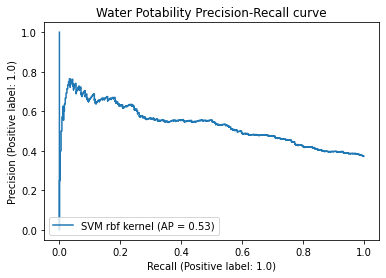
\includegraphics[width=\textwidth]{../images/pr-svm}
			\caption*{PR curve}
			\label{fig:knn}
		\end{subfigure}
		\begin{subfigure}[b]{0.35\textwidth}
			\centering
			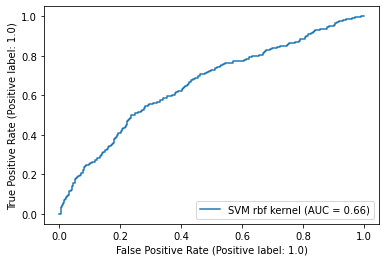
\includegraphics[width=\textwidth]{../images/roc-svm}
			\caption*{ROC curve}
			\label{fig:three sin x}
		\end{subfigure}
	\end{figure}
	\clearpage
	\section*{Apartat A}
	A continuació veurem la distribucio de la potabilitat segons els atributs. És molt difícil que puguem tenir un bon model, ja que tots els punts estan molt solapats i els atributs tenen poca correlació entre ells.\\
\begin{figure}[!h]
	\centering
	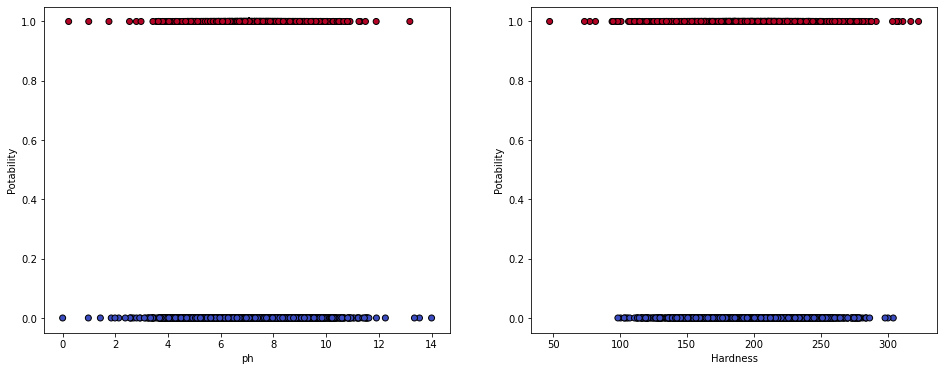
\includegraphics[width=0.7\linewidth]{../images/aa-ph}
	\caption*{pH i Hardness}
	\label{fig:aa-ph}
\end{figure}
\begin{figure}[!h]
	\centering
	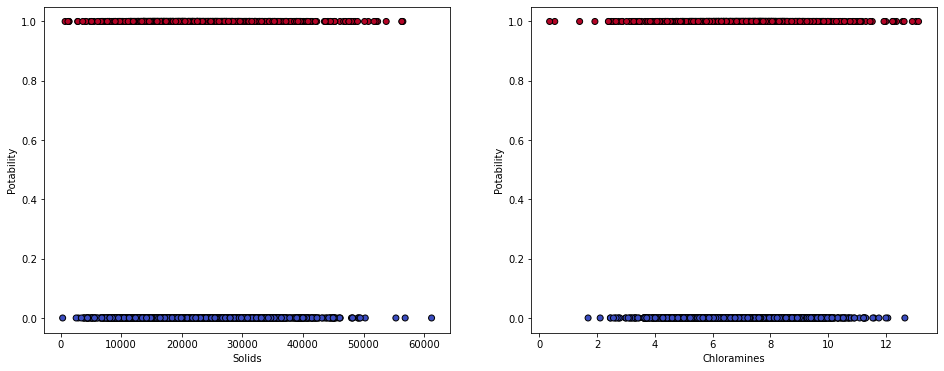
\includegraphics[width=0.7\linewidth]{../images/aa-solids}
	\caption*{Solids i Cloramines}
	\label{fig:aa-ph}
\end{figure}
\begin{figure}[!h]
	\centering
	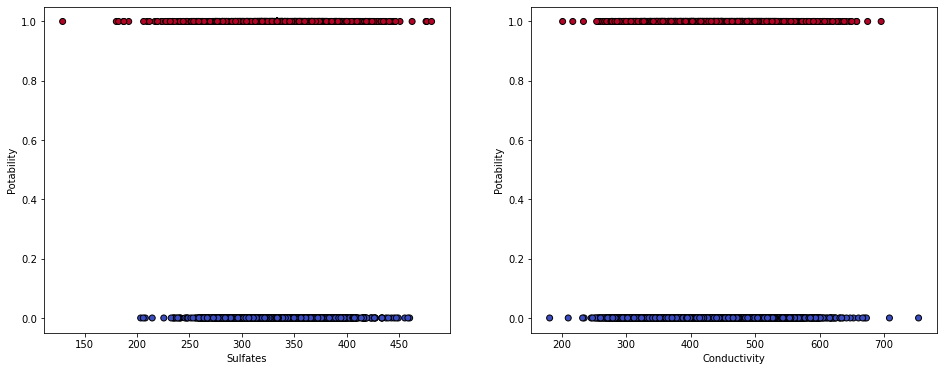
\includegraphics[width=0.7\linewidth]{../images/aa-sulfats}
	\caption*{Sulfats i Conductivitat}
	\label{fig:aa-ph}
\end{figure}
\clearpage
\begin{figure}[!h]
	\centering
	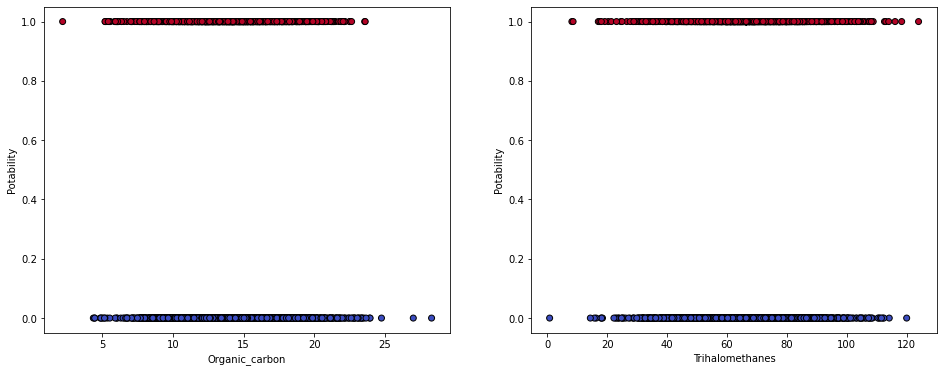
\includegraphics[width=0.7\linewidth]{../images/aa-organic-carbon}
	\caption*{Organic Carbon i Trihalomethanes}
	\label{fig:aa-ph}
\end{figure}
\begin{figure}[!h]
	\centering
	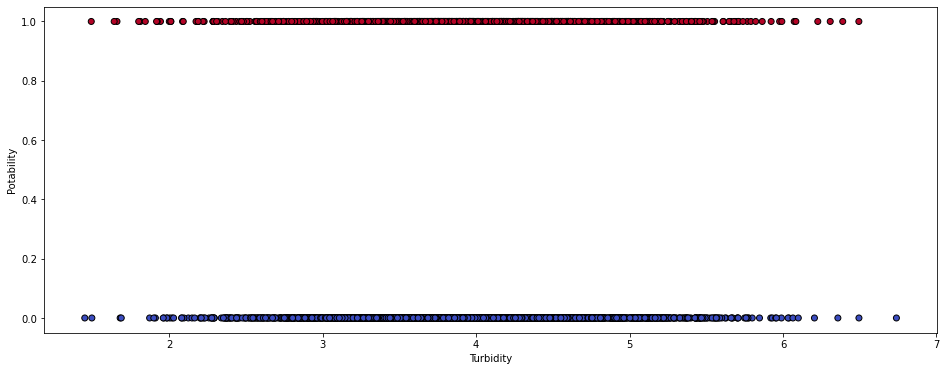
\includegraphics[width=0.7\linewidth]{../images/turbidity}
	\caption*{Turbidity}
	\label{fig:aa-ph}
\end{figure}
\begin{figure}[!h]
	\centering
	\begin{subfigure}[b]{0.4\textwidth}
		\centering
		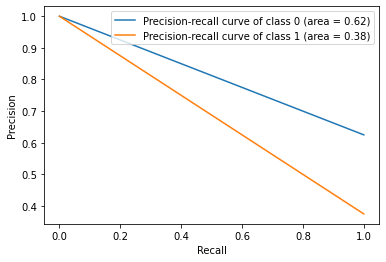
\includegraphics[width=\textwidth]{../images/bb1}
		\caption*{PR curve amb SVM rbf}
		\label{fig:knn}
	\end{subfigure}
	\begin{subfigure}[b]{0.4\textwidth}
		\centering
		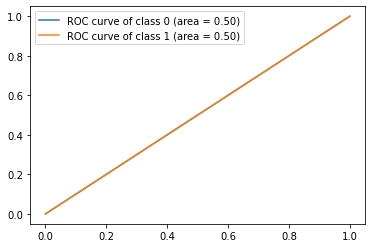
\includegraphics[width=\textwidth]{../images/bb2}
		\caption*{ROC curve amv SVM rbf}
		\label{fig:three sin x}
	\end{subfigure}
\end{figure}
\clearpage
També hem vist els efectes de variar els valors de regularització (C, degree i $\gamma$):\\
\begin{figure}[!h]
	\centering
	\begin{subfigure}[b]{0.4\textwidth}
		\centering
		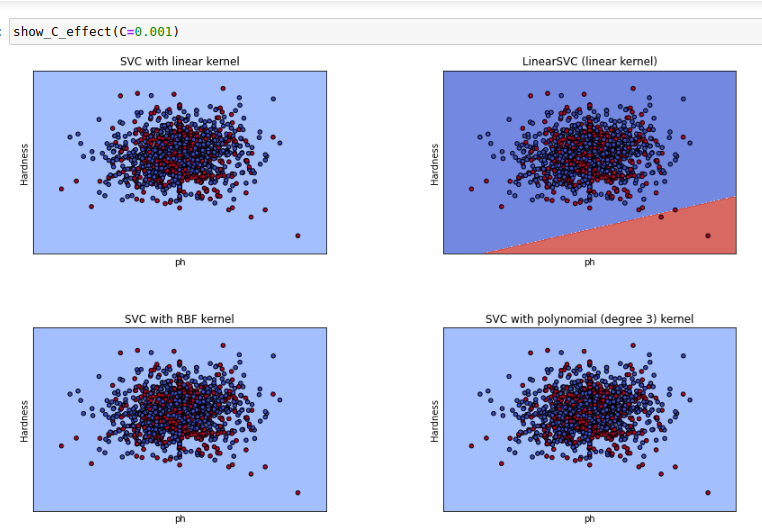
\includegraphics[width=\textwidth]{../resultats/C=0.001}
		\caption*{C=0.001}
		\label{fig:knn}
	\end{subfigure}
	\begin{subfigure}[b]{0.4\textwidth}
		\centering
		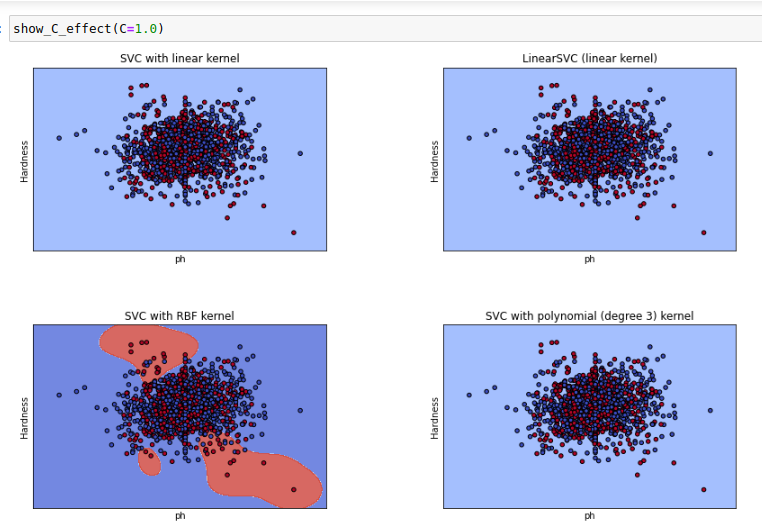
\includegraphics[width=\textwidth]{../resultats/C=1}
		\caption*{C=1}
		\label{fig:three sin x}
	\end{subfigure}
\end{figure}
\begin{figure}[!h]
	\centering
	\begin{subfigure}[b]{0.4\textwidth}
		\centering
		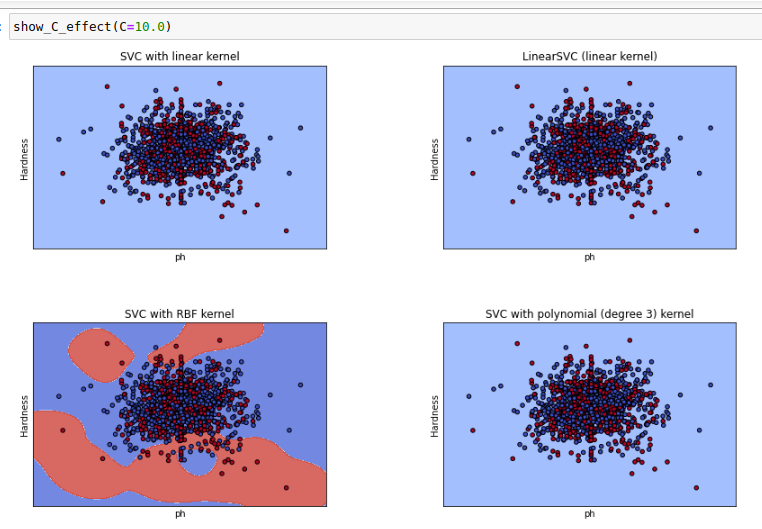
\includegraphics[width=\textwidth]{../resultats/C=10}
		\caption*{C=10}
		\label{fig:knn}
	\end{subfigure}
	\begin{subfigure}[b]{0.4\textwidth}
		\centering
		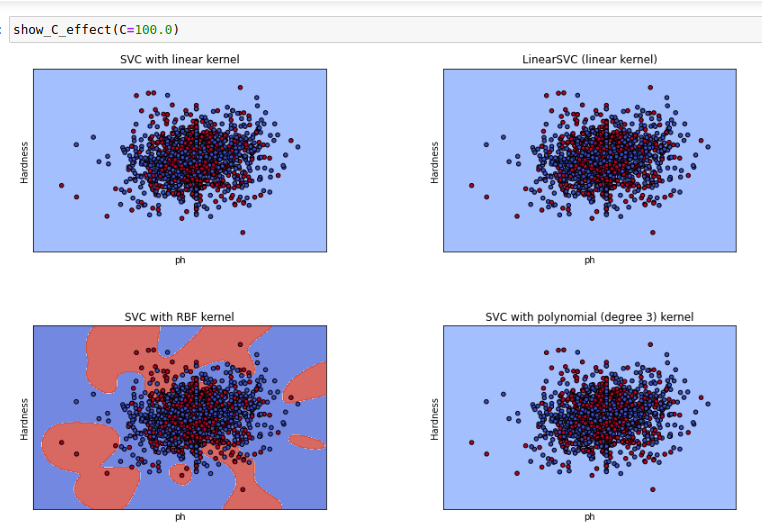
\includegraphics[width=\textwidth]{../resultats/C=100}
		\caption*{C=100}
		\label{fig:three sin x}
	\end{subfigure}
\end{figure}
\begin{figure}[!h]
	\centering
	\begin{subfigure}[b]{0.25\textwidth}
		\centering
		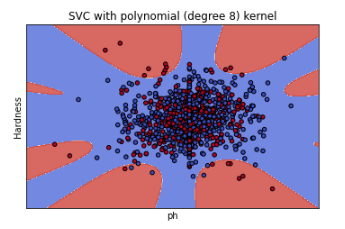
\includegraphics[width=\textwidth]{../resultats/degree=8}
		\caption*{degree=8}
		\label{fig:knn}
	\end{subfigure}
	\begin{subfigure}[b]{0.25\textwidth}
		\centering
		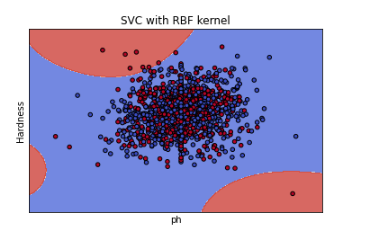
\includegraphics[width=\textwidth]{../resultats/gamma = 0.1}
		\caption*{$\gamma$=0.1}
		\label{fig:three sin x}
	\end{subfigure}
	\begin{subfigure}[b]{0.25\textwidth}
		\centering
		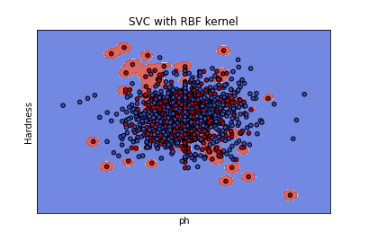
\includegraphics[width=\textwidth]{../resultats/gamma = 10}
		\caption*{$gamma$=10}
		\label{fig:three sin x}
	\end{subfigure}
\end{figure}
\end{document}